\section{Simulation and results}\label{sec:simulation}
\subsection{Cyber system security evaluation:} 
The three substation cyber system models are designed as discussed in Section~\ref{sec:technical}. The SSH vulnerability is considered to be a zero day type and the CVSS score for it is $0.8$. For the other vulnerabilities, the vulnerability database is used to determine the CVSS scores~\cite{nist1,nist2,ftp,http,ssh}. The CVSS scores for the vulnerabilities are listed in Table~\ref{tbl:CVSS}.
\begin{table}[ht]
	\centering
	\small
	\caption{CVSS scores of vulnerabilities}
	\label{tbl:CVSS}
	\begin{tabular}{|c|c|c|c|c|c|c|c|}
		\hline
		\textbf{Vulnerability} & ssh & ftp & http & xss & bof & exe & dos \\ \hline
		\textbf{CVSS score}    & 0.8 & 6.4 & 9.3  & 4.5 & 6.8 & 10.0& 5.0 \\ \hline
	\end{tabular}
\end{table}

\begin{figure}[htbp]
	\centering
	\begin{subfigure}{0.24\textwidth}
	\centering
	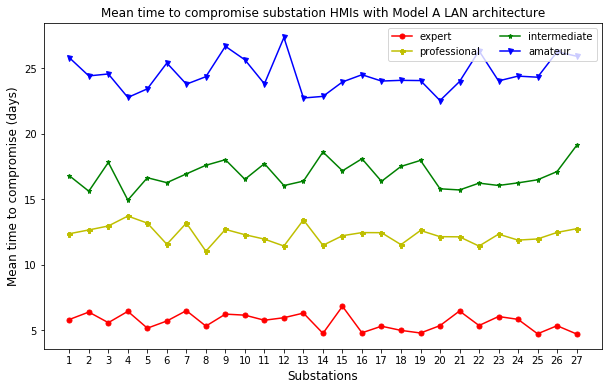
\includegraphics[width=\textwidth]{fig-resultA.png}
	\caption{}
	\label{sfig:result-A}
	\end{subfigure}
	\begin{subfigure}{0.24\textwidth}
	\centering
	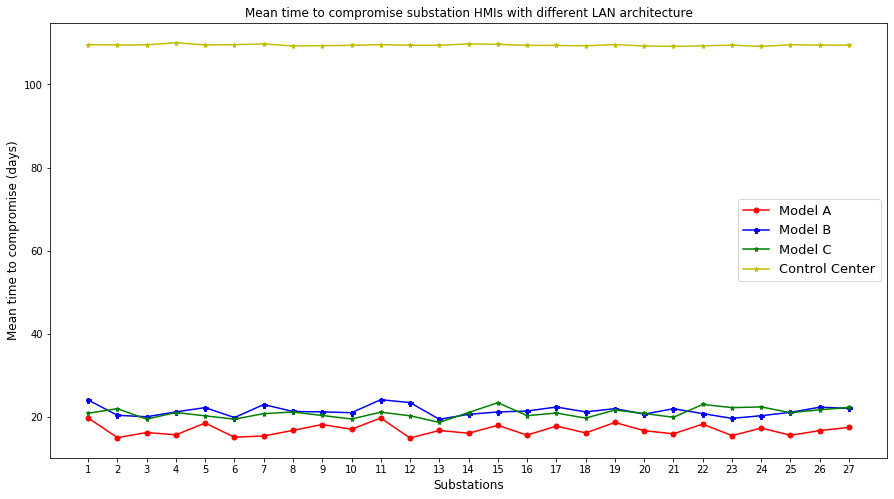
\includegraphics[width=\textwidth]{figs/fig-compare-model.png}
	\caption{}
	\label{sfig:result-compare}
	\end{subfigure}
	\caption{Comparison of mean time to compromise different LAN models with different skill level of intruder and different security level of model.}
	\label{fig:result-1}
\end{figure}
From Fig.~\ref{sfig:result-A}, it is evident that the time taken by an expert adversary to compromise an HMI is the least and an amateur adversary takes the longest to compromise the HMIs in the substation. Similar results can be observed for other substation LAN architectures and control center model. Fig.~\ref{sfig:result-compare} compares the security of different substation LAN architectures. We see that the mean time to compromise a HMI in LAN architecture A for an adversary with intermediate skill level is the least. Therefore, LAN models B and C are more secure than model A. Furthermore, The control center cyber system has a higher security than the substation LAN models.

\subsection{Risk assessment of cyber-physical system:} 
Fig.~\ref{sfig:impact1} shows the impact of a cyber-physical attack on substation HMIs in the IEEE 39-bus power system. There are $27$ substations as shown in Fig.~\ref{sfig:ieee-39}. The LAN architecture for each substation is randomly selected from the three models (Model A, Model B and Model C). The physical impact of a cyber attack at a substation is the mean impact of all possible contingencies if the HMI of the substation is compromised. Fig.~\ref{sfig:impact2} shows the impact of a cyber-physical attack on control center application server in the IEEE 39-bus power system. Comparing this type of attack with the attack on substation, it is observed that the LAN models of substations are more vulnerable than the control center SCADA system.
\begin{figure}[htbp]
	\centering
	\begin{subfigure}{0.48\textwidth}
	\centering
	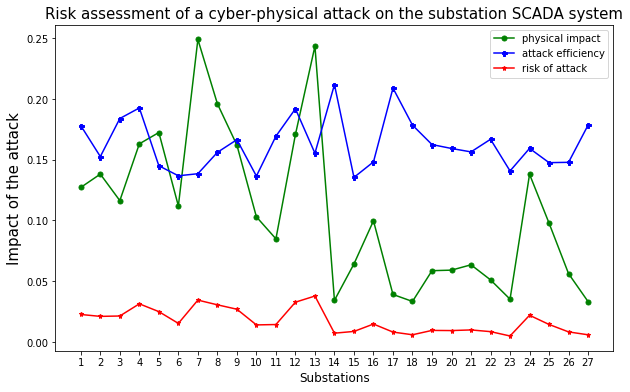
\includegraphics[width=\textwidth]{fig-impact1.png}
	\caption{Impact of cyber-physical attack on substation HMIs}
	\label{sfig:impact1}
	\end{subfigure}
	\begin{subfigure}{0.48\textwidth}
	\centering
	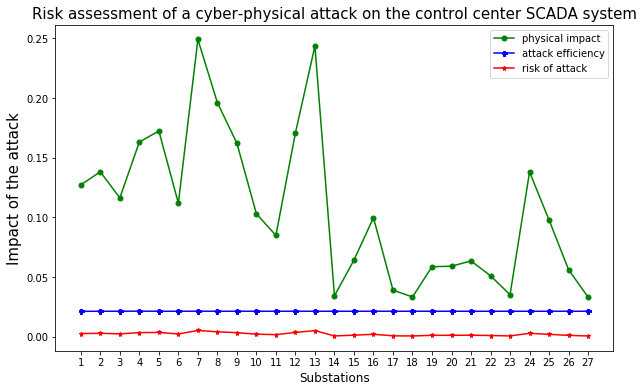
\includegraphics[width=\textwidth]{fig-impact2.png}
	\caption{Impact of cyber-physical attack on control center SCADA}
	\label{sfig:impact2}
	\end{subfigure}
	\caption{We compare the impact of cyber-[hysical attacks on different LAN architectures}
	\label{fig:result-2}
\end{figure}


